\chapter{SMO算法}

我们看到了如何使用凸优化包来解决SVM优化问题。然而,在实践中,我们将使用一种专门为快速解决这个问题而创建的算法:SMO(序列最小优化)算法。大多数机器学习库使用SMO算法或其他变体。

SMO算法将解决以下优化问题:

\begin{gather*}
\begin{align*}
\underset{\alpha}{\text{minimize}} \quad & \frac{1}{2}\sum_{i=1}^m\sum_{j=1}^m \alpha_i \alpha_j y_i y_j K(\mathbf{x}_i \cdot \mathbf{x}_j) -\sum_{i=1}^m \alpha_i \\
subject\ to \quad & 0 \leq \alpha_i \leq C,\text{for any }i=1,\dots,m \\
& \sum_{i=1}^m \alpha_i y_i = 0
\end{align*}
\end{gather*}

它是我们在第5章中看到的软间隔公式的核化版本。我们试图最小化的目标函数可以用Python编写(代码37):

\emph{代码37}

\begin{lstlisting}[language=python]
def kernel(x1, x2): 
    return np.dot(x1, x2.T) 

def objective_function_to_minimize(X, y, a, kernel): 
    m, n = np.shape(X) 
    return 1 / 2 * np.sum([a[i] * a[j] * y[i] * y[j]* kernel(X[i, :], X[j, :]) for j in range(m) for i in range(m)])\ - np.sum([a[i] for i in range(m)])
\end{lstlisting}

这和我们使用CVXOPT解决的问题是一样的。为什么我们需要另一种方法?因为我们希望能够在大数据集上使用支持向量机,而使用凸优化包通常涉及到矩阵操作,随着矩阵大小的增加,这些操作需要花费大量时间,或者由于内存限制而变得不可能。创建SMO算法的目标是比其他方法更快。

\section{SMO背后的理念}
当我们尝试解决SVM优化问题时,只要我们满足约束条件,我们可以自由地改变的$\alpha$值。我们的目标是修改$\alpha$,使目标函数最终返回最小的可能值。在这种情况下,给定一个拉格朗日乘子向量$\alpha=(\alpha_1,\alpha_2,\dots,\alpha_m)$,我们可以改变任意值$\alpha_i$,直到我们达到目标。

SMO背后的思想非常简单:我们将解决一个更简单的问题。也就是说,给定一个向量$\alpha=(\alpha_1,\alpha_2,\dots,\alpha_m)$,我们只允许自己改变$\alpha$的两个值,例如,$\alpha_3$和$\alpha_7$。我们将改变它们,直到目标函数达到给定的最小值。然后,我们将选择另外两个alpha并更改它们,直到函数返回其最小值,以此类推。如果我们继续这样做,最终会得到原问题的目标函数的最小值。

> 注:如果仅修改一个$\alpha_i$的值,就会违反约束条件$\sum\limits_{i=1}^m \alpha_i y_i = 0$,所以要两个一起修改。

SMO解决了一系列简单的优化问题

\section{How did we get to SMO}

这种解决几个更简单的优化问题的想法并不新鲜。1982年,Vapnik提出了一种称为“分块(chunking)”的方法,将原始问题分解成一系列更小的问题(Vapnik V., 1982)。让事情发生变化的是,1997年,Osuna等人证明了只要我们加入至少一个违反KKT条件的例子,求解一系列子问题将保证收敛(Osuna, Freund, \& Girosi, 1997)。

利用这个结果,一年后,也就是1998年,Platt提出了SMO算法。

\section{SMO为什么快}

SMO方法的最大优点是我们不需要QP求解器来求解两个拉格朗日乘子的问题——它可以解析求解。因此,它不需要存储一个巨大的矩阵,从而导致机器内存出现问题。此外,SMO使用了几种启发式算法来加快计算速度。

\section{SMO算法 }

SMO算法由三部分组成:

* 根据启发式方法选择第一个拉格朗日乘子 
* 根据启发式方法选择第二个拉格朗日乘子 
* 根据选择的两个乘子,用代码求优化问题的解析解

> Tip: 该算法的Python实现可在附录B: SMO算法中获得。本节中的所有代码清单都摘自本附录,并不是单独运行的。

\subsection{解析解}

在算法的开始前,我们把向量$\alpha(\alpha_1,\alpha_2,\dots,\alpha_m)$初始化为0,即$\alpha_i=0,for\ all\ i=1,\dots,m$。其思想是从这个向量中选择两个元素,我们将其命名为$\alpha_1$和$\alpha_2$,并更改它们的值,以使约束条件仍然满足。

第一个约束条件$0 \leq \alpha_i \leq C ,for\ all\ i=1,\dots,m$意味着$0 \leq \alpha_1 \leq C,0 \leq \alpha_2 \leq C$。这就是为什么我们选择图\ref{figure50}中蓝色框内的值(其中$C=5$)

第二个约束是一个线性约束$\sum\limits_{i=1}^m \alpha_i y_i = 0$。它的取值范围位于红色对角线上,并且之前被选中的乘子$\alpha_1$和$\alpha_2$应该有不同的标签($y_1 \neq y_2$)。

\begin{figure}[ht]
	\centering
	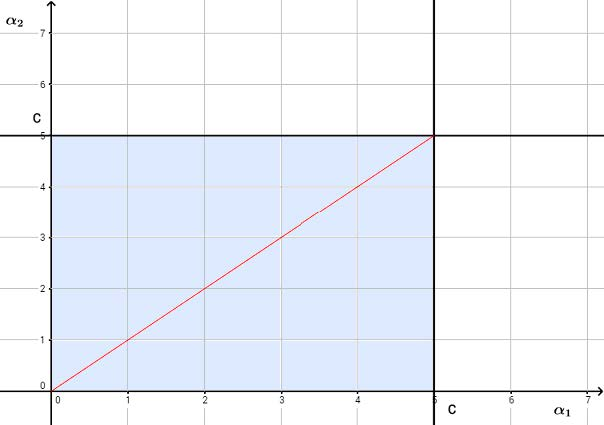
\includegraphics{figure50}
	\caption{可行集是蓝色区域的对角线}
	\label{figure50}
\end{figure}

一般来说,为了避免打破线性约束,我们必须改变乘子,像这样:
\begin{gather*}
\alpha_1 y_1 + \alpha_2 y_2 = constant = \alpha_1^{old} y_1 + \alpha_2^{old} y_2
\end{gather*}

我们不会深入分析问题是如何解决的细节,因为它在(Cristianini \& shaw - taylor, 2000)和(Platt J. C., 1998)做得很好。

记住,有一个公式来计算新的$\alpha_2$:
\begin{gather*}
\alpha_2^{new} = \alpha_2 + \frac{y_2(E_1-E_2)}{K(\mathbf{x}_1,\mathbf{x}_1)+K(\mathbf{x}_2,\mathbf{x}_2)-2K(\mathbf{x}_1,\mathbf{x}_2)}
\end{gather*}

其中$E_i = f(\mathbf{x}_i)-y_i$是假设函数的输出和样本标签之间的差值。$K$是核函数。我们还计算了适用于$\alpha_2^{new}$的边界;它不能小于下界,也不能大于上界,否则会违反约束。在这种情况下$\alpha_2^{new}$被修剪掉了。

> 注:这里的修剪的意思大致如下: 
\begin{lstlisting}[language=python]
ifa>C:
    a = C
elif a<0:
    a = 0
\end{lstlisting}

一旦我们有了这个新值,我们就用它来计算$\alpha_1$的新值:
\begin{gather*}
\alpha_1^{new} = \alpha_1^{old}+y_1 y_2 (\alpha_2^{old}-\alpha_2^{new})
\end{gather*}

\subsection{理解第一个启发式选择}

第一个启发式背后的想法非常简单:每次 SMO 检查一个样本时,它都会检查是否违反了 KKT 条件。 回想一下,至少有一个样本违反了KKT条件(注:如果全都满足KKT条件,那就是最优解了,不用再求了)。 如果满足条件,则尝试另一个样本。 因此,如果有数百万个示例,而其中只有少数违反了 KKT 条件,它将花费大量时间检查无用的示例。 为了避免这种情况,该算法将时间集中在拉格朗日乘数不等于$0$或不等于$C$的样本上,因为它们最有可能违反条件(代码 38)。

\emph{代码38}

\begin{lstlisting}[language=python]
def get_non_bound_indexes(self): 
    return np.where(np.logical_and(self.alphas > 0, self.alphas < self.C))[0] 
    
# First heuristic: loop over examples where alpha is not 0 and not C 
# they are the most likely to violate the KKT conditions 
# (the non-bound subset). 
def first_heuristic(self): 
    num_changed = 0 
    non_bound_idx = self.get_non_bound_indexes() 
    
    for i in non_bound_idx: 
        num_changed += self.examine_example(i) 
    return num_changed
\end{lstlisting}

由于解析解问题涉及两个拉格朗日乘数,有可能一个约束乘数(其值在$0$和$C$之间)已经违反了KKT条件。这就是主程序在所有样本和非边界(non-bound)子集之间交替的原因(代码39)。注意,当不再有进展时,算法结束

\subsection{理解第二个启发式选择}

第二种启发式选择的目标是选择变化最大的拉格朗日乘子。

怎么更新$\alpha_2$呢,我们使用之前的公式:
\begin{gather*}
\alpha_2^{new} = \alpha_2 + \frac{y_2(E_1-E_2)}{K(\mathbf{x}_1,\mathbf{x}_1)+K(\mathbf{x}_2,\mathbf{x}_2)-2K(\mathbf{x}_1,\mathbf{x}_2)}
\end{gather*}

记住,在这个例子中,我们已经选择了$\alpha_1$值。我们的目标是选出那些将会使$\alpha_2$最大改变的。这个公式可以改写为:

\begin{gather*}
\alpha_2^{new} = \alpha_2 + step \\
step = \frac{y_2(E_1-E_2)}{K(\mathbf{x}_1,\mathbf{x}_1)+K(\mathbf{x}_2,\mathbf{x}_2)-2K(\mathbf{x}_1,\mathbf{x}_2)}
\end{gather*}

所以,为了从几个$\alpha_2$中选出最好的$\alpha_2$,我们需要计算每个$\alpha_i$的步长并选择步长最大的那个。这里的问题是每一步我们需要调用核函数$K$三次,这代价很高。Platt没有这么做,而是提出了以下近似:
\begin{gather*}
step \approx |E_1 -E_2|
\end{gather*}
因此,当$E_1$为正时,那么选择最小的$E_i$作为$E_2$;如果$E_1$为负,选择最大$E_i$作为$E_2$。

在代码40的方法\colorbox{lightgray}{second\_heuristic}中可以看到这种选择。

\emph{代码40}

\begin{lstlisting}[language=python]
def second_heuristic(self, non_bound_indices): 
    i1 = -1 
    if len(non_bound_indices) > 1: 
        max = 0 

    for j in non_bound_indices: 
        E1 = self.errors[j] - self.y[j] 
        step = abs(E1 - self.E2) # approximation 
        if step > max: 
            max = step 
            i1 = j 
        return i1 
        
def examine_example(self, i2): 
    self.y2 = self.y[i2] 
    self.a2 = self.alphas[i2] 
    self.X2 = self.X[i2] 
    self.E2 = self.get_error(i2) 
    
    r2 = self.E2 * self.y2 
    
    if not((r2 < -self.tol and self.a2 < self.C) or (r2 > self.tol and self.a2 > 0)): 
        # The KKT conditions are met, SMO looks at another example. 
        return 0 
    
    # Second heuristic A: choose the Lagrange multiplier that 
    # maximizes the absolute error. 
    non_bound_idx = list(self.get_non_bound_indexes()) 
    i1 = self.second_heuristic(non_bound_idx) 
    
    if i1 >= 0 and self.take_step(i1, i2): 
        return 1 
        
    # Second heuristic B: Look for examples making positive 
    # progress by looping over all non-zero and non-C alpha, 
    # starting at a random point. 
    if len(non_bound_idx) > 0: 
        rand_i = randrange(len(non_bound_idx)) 
        for i1 in non_bound_idx[rand_i:] + non_bound_idx[:rand_i]: 
            if self.take_step(i1, i2): 
                return 1 
                
    # Second heuristic C: Look for examples making positive progress 
    # by looping over all possible examples, starting at a random
    # point. 
    rand_i = randrange(self.m) 
    all_indices = list(range(self.m)) 
    for i1 in all_indices[rand_i:] + all_indices[:rand_i]: 
        if self.take_step(i1, i2): 
            return 1 
    
    # Extremely degenerate circumstances, SMO skips the first example. 
    return 0
\end{lstlisting}

\section{总结}

理解SMO算法可能很困难,因为这里有很多代码是出于性能原因,或者是为了处理特定的退化情况。然而,其核心的算法不难,而且比凸优化求解速度更快。随着时间的推移,人们已经发现了新的启发式算法来改进该算法,而且像LIBSVM这样的流行库使用了类似于smo的算法。注意,即使这是解决SVM问题的标准方法,也存在其他方法,如梯度下降和随机梯度下降(stochastic gradient descent,SGD),这用于在线学习和处理巨大的数据集。

了解SMO算法如何工作将帮助您确定它是否是您想要解决的问题的最佳方法。我强烈建议你自己试试。在斯坦福CS229课程中,你可以找到一个\href{http://cs229.stanford.edu/materials/smo.pdf)的描述,这是一个很好的开始。然后,在序列最小化(Platt J. C., 1998}{简化版算法},你可以阅读算法的完整描述。附录B中提供的Python代码是用本文的伪代码编写的,并在注释中指出代码的哪些部分对应于本文中的哪些方程。